\section{Durchführung}
\label{sec:Durchführung}
\subsection{Bestimmung der Zeitkonstante}
Zur Bestimmung der Zeitkonstante wird die Schaltung aus \autoref{fig:schaltung1} verwendet. Die Auf - und Entladung des Kondensators wird 
hier, wie zu sehen, über eine Rechteckspannung verwirklicht. Die Aufladekurve wird auf einem digitalen Oszilloskop dargestellt. Anschließend
werden mittels der Cursorfunktion des Oszilloskops mindestens 10 Zusammmenhänge zwischen Zeitpunkt der Ladung und der dortigen Spannung
auf dem Kondensator aufgenommen. Zu Beachten ist dabei die Position des Spannungsnullpunktes, welche auf dem Bildschirm bekannt sein muss.
\begin{figure}
    \centering
    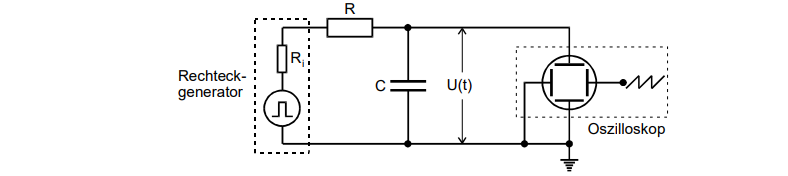
\includegraphics[width=\textwidth]{content/schaltung1.png}
    \caption{Schaltung zur Bestimmung der Zeitkonstante des Relaxationsvorgangs \cite[281]{v353}.}
    \label{fig:schaltung1}
\end{figure}
\subsection{Bestimmung der frequenzabhängigen Amplitude und Phasendifferenz}
Zur Bestimmung der Frequenzabhängigkeit der Amplitude der Kondersatorspannung wird die Schaltung, welche in \autoref{fig:schaltung2} zu 
sehen ist, verwendet, wobei der zweite Kanal des Oszilloskops zunächst nicht benötigt wird.
Mittels des Sinusgenerators lassen sich Sinusschwingungen verschiedener Frequenzen erzeugen und auf die Schaltung ausgeben. Das Oszilloskop 
zeigt dann wieder die Spannung des Kondensators an, dessen Amplitude mit der Cursorfunktion des Oszilloskops ausgemessen wird. Insgesamt 
werden pro Zehnerpotenz, im Bereich von $10 \, \symup{Hz} - 10000 \, \symup{Hz}$, Messungen für zehn verschiedene Frequenzen durchgeführt.
Die Bestimmung der Phasendifferenz der Kondensatorspannung erfolgt analog zur Messung der Amplituden. Dieses Mal werden beide Kanäle 
des Oszilloskops aus \autoref{fig:schaltung2} verwendet; der erste Kanal zeigt nun die Kondensatorspannung, während der zweite Kanal
die Spannung des Generators widergibt. Der Abstand der Nulldurchgänge der beiden Kurven wird wieder mittels der Cursorfunktion ermittelt.
Die verwendeten Frequenzen, in deren Abhängigkeit die Phasendifferenz gemessen wird, müssen für die anschließende Überprüfung des Integratorverhaltens
die selben Werte sein, wie schon bei der Messung der Amplitude. Zu Beachten ist hierbei noch, dass beide Sinuskurven symetrisch zur gleichen
X-Achse liegen. 
\begin{figure}
    \centering
    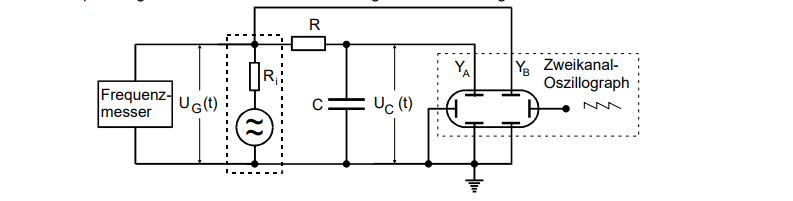
\includegraphics[width=\textwidth]{content/schaltung2.png}
    \caption{Schaltung zur Bestimmung der Phasendifferenz und der Amplitude der Kondensatorspannung bei angelegter Wechselspannung und zur Überprüfung der Intergratorfunktion des RC-Kreises \cite[282]{v353}.}
    \label{fig:schaltung2}
\end{figure}
\subsection{Überprüfung der Intergratorfunktion des RC-Kreises}
Hier wird wieder die Schaltung aus \autoref{fig:schaltung2} verwendet. Der Funktionengenerator wird nacheinander auf eine Rechteck-, Sinus-
beziehunsweise Dreieckspannung eingestellt. Auf dem Bildschirm sind nun die generierte Spannung, sowie die durch den RC-Kreis intergierte
Spannung zu sehen. Zum späteren Vergleich werden die Anzeigen als Thermodrucke aufgenommen.
